\documentclass[11pt]{article}
\usepackage[utf8]{inputenc}
\usepackage[english]{babel}
\usepackage[font=small,labelfont=bf]{caption}
\usepackage{geometry}
\usepackage[sort&compress]{natbib}
\usepackage{amsmath}
\usepackage{pxfonts}
\usepackage{graphicx}
\usepackage{setspace}
\usepackage{hyperref}
\usepackage{lineno}
\usepackage{booktabs}

\doublespacing

\title{A Stylometric Application of Large Language Models}

\author{Harrison F. Stropkay, Jiayi Chen, Daniel N. Rockmore, and Jeremy R. Manning\\
Dartmouth College \\
Hanover, NH 03755, USA \\
\texttt{\{harrison.f.stropkay.25, jiayi.chen.gr, }\\\texttt{daniel.n.rockmore, jeremy.r.manning\}@dartmouth.edu}}

\begin{document}
\maketitle

\begin{abstract}

We show that large language models (LLMs) can be used to distinguish the
writings of different authors. Specifically, an individual model, trained on
the works of one author, will predict held-out text from that author more
accurately than held-out text from other authors. We suggest that, in this way,
a model trained on one author's works embodies the unique writing style of that
author. We first demonstrate our approach on books written by eight different
(known) authors. We also use this approach to confirm R. P. Thompson's
authorship of the well-studied 15\textsuperscript{th} book of the \textit{Oz}
series, originally attributed to F. L. Baum.

\end{abstract}

\section{Introduction}

Herein we introduce {\em predictive comparison}, a new LLM-based relative
stylometric measure. It derives from a simple idea, that if an LLM can be
trained to write like---i.e., in the style of---a given author by training on
their work~\citep[e.g., ][]{Mikr25}, then the degree to which such a model can
predict another author's work could be a measure of stylistic similarity. This
approach builds upon a growing body of work applying language models to
authorship attribution~\citep{HuanEtal25,UcheEtal20}, extending established
information-theoretic methods in stylometry~\citep{JuolBaay05,ZhaoEtal06}.

Recent work has demonstrated the effectiveness of using perplexity and
cross-entropy loss from fine-tuned language models for authorship
attribution~\citep{HuanEtal25}, achieving state-of-the-art performance on
standard benchmarks. Unlike traditional stylometric approaches that rely on
hand-crafted features such as function word frequencies~\citep{MostWall63} or
syntactic patterns~\citep{Holm98}, lage language models can capture complex,
hierarchical patterns in authorial style~\citep{FabiEtal20}. This shift from
explicit feature engineering to learned representations parallels broader
trends in computational literary analysis~\citep{More00,UndeEtal19} and digital
humanities~\citep{HughEtal12}.

In this paper we show, using a small set of authors and their works, that large
language models capture author-specific writing patterns. Our method differs
from related approaches~\citep{Reza25} in scale (we use entire books rather
than individual sentences) and in our reliance solely on cross-entropy loss as
a measure of stylometric distance. This in turn suggests a notion of
stylometric distance derived from the cross-entropy loss assigned to held-out
texts by models trained on known works of different authors. We believe this
approach could be of use in considering questions of authorial influence and
stylistic evolution~\citep{HughEtal12}. Lastly, this further suggests a
literary authentication tool~\citep[a common use of stylometric techniques;
][]{MostWall63,MostWall84,NiloBino03,Juol08} that would assign an unknown or
contested work to the model (and author) under which predictive comparison
generates the smallest loss. We illustrate this on the well-known attribution
problem of the 15\textsuperscript{th} book in the \emph{Oz} series, confirming
what is now the accepted attribution. 

\section{Methods}

In this section, we outline our methodology for identifying stylometric
signatures using large language models. For each selected author, we train a
GPT-2 model~\citep{RadfEtal19} on that author's corpus. We then use the trained
model to compute the cross-entropy loss on held-out texts from both the target
author and each of the other authors in the dataset. By comparing these losses,
we assess whether the model captures author-specific stylistic patterns: a
model trained on a given author should exhibit lower loss when predicting that
author's own texts as compared to the texts of others.

\subsection{Data and preprocessing \label{sec:data}}

We consider a dataset comprising books by eight authors: Jane Austen, L. Frank
Baum, Charles Dickens, F. Scott Fitzgerald, Herman Melville, Rosemary Plumly
Thompson, Mark Twain, and H. G. Wells. We selected these authors because their
writings are well-represented in Project Gutenberg, are all in the public
domain, and are written in English---eliminating any potential confounds due to
translation. For each book, we pre-process the text by stripping Project
Gutenberg metadata, publisher information, illustration tags, transcriber
notes, prefaces, tables of contents, and chapter headings. We standardize
whitespace, remove non-ASCII characters, and lowercase all alphabetic
characters. Basic statistics on token lengths and the full list of books used
are provided in the Appendix.

To construct training data for each author, we randomly select one book to hold
out for evaluation and train their model using the remaining books. To ensure
fair comparisons across authors, we standardize the number of training tokens
per author by truncating each author's corpus. This token budget is determined
by removing the longest book from each author's set and then taking the
smallest of the (remaining) total token counts. For our dataset, this yields a
fixed training token budget of 643,041 tokens.

To construct a truncated corpus of 643,041 tokens for each author, we sample
one contiguous sub-sequence from each book in their training corpus (after
holding out a to-be-evaluated book). The length of the sub-sequence sampled
from book~$i$ is proportional to its original length:
\[
\text{length}_i = 643{,}041 \times \frac{\text{tokens in book
  }i}{\text{total tokens in corpus}}.
\]
The starting position of each sub-sequence is chosen uniformly at random,
ensuring the sample fits within the book's bounds. Finally, we shuffle and then
concatenate the sampled sub-sequences from each book, resulting in a single
643,041-token training sequence for each author. This process is repeated for
each of 10 random seeds, yielding 10 different training corpora for each
author.

\subsection{Model architecture, training, and evaluation}

For each author, we train GPT-2 language models from scratch using the
\texttt{GPT2LMHeadModel} class from the Hugging Face \texttt{Transformers}
library with custom architecture settings: a context window of 1024 tokens, an
embedding dimension of 128, 8 transformer layers, and 8 attention heads per
layer. We fit each model using the AdamW optimizer~\citep{LoshHutt17} with a
learning rate of $5 \times 10^{-5}$ to minimize the cross-entropy loss on the
training data. We train models using a causal language modeling objective,
whereby the model iteratively predicts the next token in the sequence given all
of the previous tokens in the same training sequence.

We construct training samples by sampling 1024-token chunks from the truncated
corpus for the given author and random seed (constructed as described above,
using contiguous sub-sequences selected from all but one of their books). Each
training epoch consists of 40 batches, each containing 16 sequences of 1024
tokens. This results in a total of 655,360 tokens per epoch. We continue
training until the cross-entropy loss falls to 3.0 or lower. (We decided on
this threshold after taking random draws from the models trained on Baum's and
Thompson's \textit{Oz} books and manually inspecting the quality of the
resulting samples.) Training to a fixed loss threshold (e.g., as opposed to
training for a fixed number of epochs) enables us to fairly compare model
performance across authors, which is the central component of our stylometric
analyses.

We evaluate the models using the held-out book from the corresponding author.
We partition the held-out book into 1024-token chunks to ensure that each token
in the evaluation set contributes equally to the computed loss. We repeat the
full process (of selecting a held-out book at random and training the model
using randomly selected samples from the remaining books) using 10 different
random seeds. This approach enables us to assess the robustness of our results
and to ensure that the models are not overfitting to a specific book or random
sample.

\begin{figure*}[t]
  \centering
  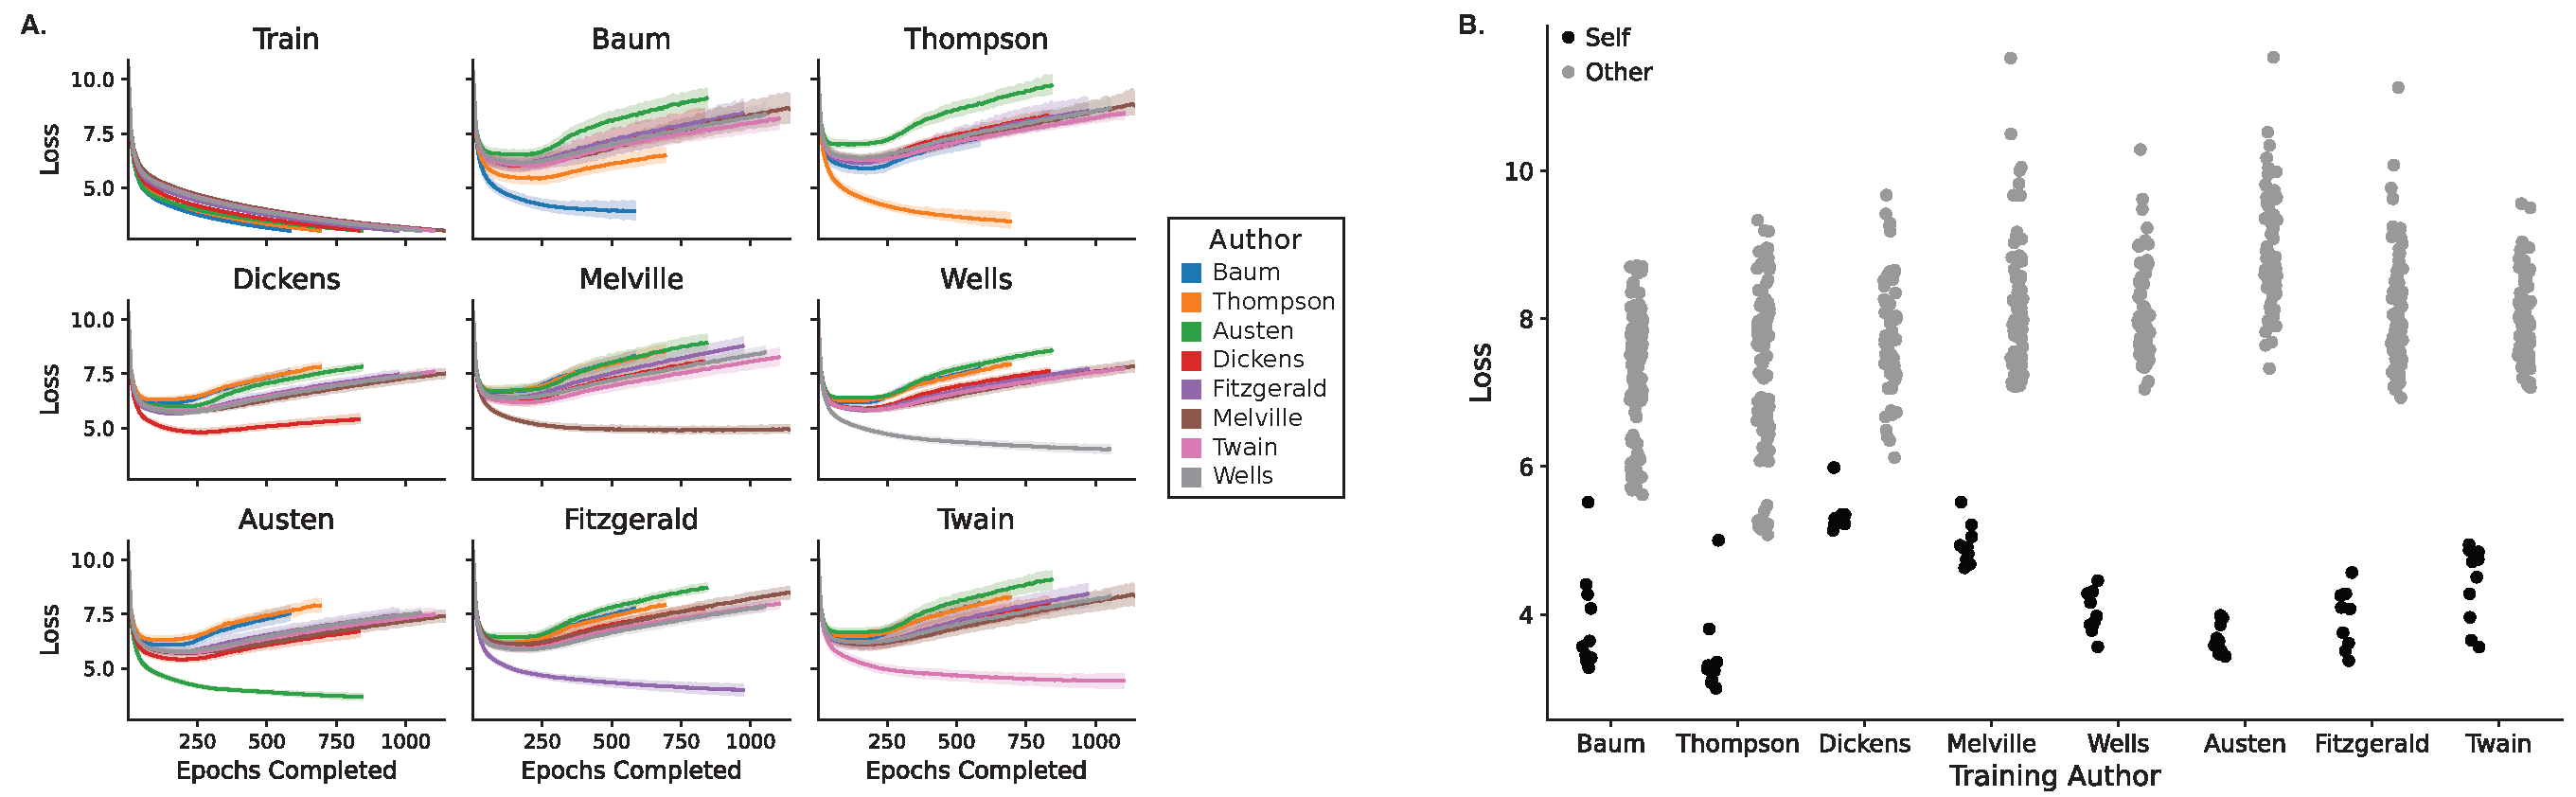
\includegraphics[width=\textwidth]{figs/loss_all_authors.pdf}


  \caption{\textbf{Cross-entropy loss across models and
      authors.}\textbf{A.} Average cross-entropy loss on
    \textit{Train}ing data and held-out test data from each author,
    plotted as a function of the number of training epochs. Each color
    denotes a model trained on a single author's work.  Error ribbons
    denote bootstrap-estimated 95\% confidence intervals over 10
    random seeds. \textbf{B.} Cross-entropy loss assigned to held-out
    test data by each author's model ($x$-axis). Held-out test data is
    either from the \textit{same} author (black) or from
    \textit{other} authors (gray). Each dot denotes the average loss
    (across all 1024-token chunks) for a single random seed.}
\label{fig:all-losses}
\end{figure*}

\section{Results}

\subsection{Predictive comparison testing of eight classic authors}

We carried out predictive comparison testing on eight classic authors (see
Sec.~\ref{sec:data}). The top-left sub-panel of Figure~\ref{fig:all-losses}A
(labeled ``Train'') shows the average training loss for each author's model,
computed over 10 random seeds. Training losses are comparable across models,
indicating that the models are trained to similar levels of performance. The
other sub-panels of Figure~\ref{fig:all-losses}A show the average predictive
(cross-entropy) loss, for each author's model, on held-out texts from each
author. For every author's held-out text, the model trained on the same
author's writings produces the lowest loss, indicating a clear preference for
its own author's stylistic patterns. As shown in Figure~\ref{fig:all-losses}B,
across every author we considered, and for every random seed, models trained
and tested on the same author always yield smaller losses than models trained
on one author and tested on another (i.e., for each author, the highest black
dot is always lower than the lowest gray dot in the Panel). Indeed, we achieve
perfect (100\%) classification accuracy when matching authors with held-out
texts by labeling the held-out text according to which model produces the
smallest loss.

\begin{figure*}[t]
  \centering
  \includegraphics[width=\textwidth]{figs/t_stats.pdf}


  \caption{\textbf{Same vs. other author comparisons, by
      model.}\textbf{A.} Each curve denotes, as a function of the
    number of training epochs, the the $t$-statistic from a $t$-test
    comparing the distribution of losses (across random seeds)
    assigned to held-out texts from the given author (color) versus
    held-out texts from all other authors. \textbf{B.} The average
    $t$-statistic across all eight authors, as a function of the
    number of training epochs. Error ribbons denote
    bootstrap-estimated 95\% confidence intervals across authors.}
\label{fig:t-stats}
\end{figure*}

We also wondered how many training epochs were required for the models to
reliably distinguish author styles. We compared the distributions (across
random seeds) of average cross-entropy losses for each author's model computed
for held-out text from the \textit{same} author versus for held-out text from
\textit{other} authors. Figure~\ref{fig:t-stats}A displays the $t$-values from
$t$-tests comparing these same versus other loss distributions for each of the
first 500 training epochs. For all authors except Twain, the $t$-tests yielded
$p$-values below $0.001$ after just one epoch, indicating that the models
rapidly acquire author-specific stylometric patterns. For Twain, this threshold
is crossed at epoch 47. Figure~\ref{fig:t-stats}B shows the average $t$-values
across all eight authors as a function of the number of training epochs (final
epoch: $t(9) = 20.723, p = 6.6 \times 10^{-9}$). This latter plot provides an
estimate of the performance we might expect to see in the general case (e.g.,
across a larger set of authors). Table~\ref{tab:t-tests} summarizes the results
of the $t$-tests for each author's model after training is complete.

\begin{table}[h]
\centering
\small
\begin{tabular}{lccc}
\hline
\textbf{Model} & \textbf{$t$-stat} & \textbf{df} & \textbf{$p$-value}\\
\hline
Baum        & 16.96 & 10.49 & $5.78 \times 10^{-9}$  \\
Thompson    & 21.50 & 13.60 & $6.84 \times 10^{-12}$ \\
Austen      & 47.29 & 54.75 & $4.38 \times 10^{-46}$ \\
Dickens     & 18.36 & 27.36 & $6.52 \times 10^{-17}$ \\
Fitzgerald  & 26.03 & 22.66 & $2.22 \times 10^{-18}$ \\
Melville    & 24.15 & 45.15 & $1.87 \times 10^{-27}$ \\
Twain       & 20.13 & 12.22 & $9.67 \times 10^{-11}$ \\
Wells       & 35.17 & 26.33 & $1.16 \times 10^{-23}$ \\
\hline
\end{tabular}

\caption{Each row displays the results of a $t$-test comparing the average loss
values assigned by each author's model (after training is complete) to the
author's held-out text and to the other authors' randomly sampled texts.}

\label{tab:t-tests}
\end{table}

Despite achieving perfect classification accuracy, not all authors are equally
distinctive. For example, we reasoned that authors with similar writing styles
might be more confusable (i.e., yielding relatively smaller losses for models
trained across different authors). We computed the average loss for each author
using the models trained on the other authors' texts (Fig.~\ref{fig:confusion-matrix}).
Authors with similar writing styles (e.g., Baum and Thompson) yield relatively
small losses when evaluated using models trained on the other author's texts.
In contrast, authors with more distinct writing styles (e.g., Austen and
Thompson) yield relatively large losses when evaluated using each other's
models. To illustrate these patterns, we also project the losses into a 3D
space using multidimensional scaling~\citep[MDS; ][]{Krus64} applied to the
pairwise correlations between rows of the loss matrix, excluding the diagonal
entries (i.e., the losses obtained using each author's model when applied to
their own held-out text). We observed (Fig.~\ref{fig:mds}) that Baum and
Thompson (authors of corpora largely intended to be similar) are mapped onto
nearby locations, providing some evidence that the embeddings are
``meaningful.'' We suggest that this approach might lend itself to further
exploration and consideration by literature scholars, particularly if extended
to a larger embedding space. For the purposes of our present work, however, we
provide the plot solely as a provocative demonstration.

\begin{figure*}[t]
  \centering
  \includegraphics[width=0.6\textwidth]{figs/source/loss_heatmap_ordered.pdf}


  \caption{\textbf{Confusion matrix.} The matrix displays the average cross-entropy loss assigned by models trained on each
 author's writing (column) to held-out texts from each author (row), after subtracting
 the native author's baseline loss.}
\label{fig:confusion-matrix}
\end{figure*}

\subsection{Stylometric distance~\label{sec:distance}}

As indicated by Figure~\ref{fig:mds}, predictive comparison suggests a
natural notion of distance between authorial styles. Let $L_j(i)$ denote the
average loss of a work of author $i$ for a model trained on author $j$ (entry
$i,j$ of the average loss matrix in Fig.~\ref{fig:confusion-matrix}). Let
$\overline{L_j(i)} = L_j(i)-L_j(j)$, normalizing the entries by subtracting the
native author's baseline loss. Then define the LLM-based {\em stylometric
distance}, $d(i,j) = \frac{1}{2}\left(\overline{L_j(i)} +
\overline{L_i(j)}\right)$. Thus, Figure~\ref{fig:mds} is a visualization of
the relative ``distances" among our author set.

\begin{figure*}[t]
  \centering
  \includegraphics[width=0.6\textwidth]{figs/source/3d_MDS_plot.pdf}


  \caption{\textbf{Multidimensional scaling plot.} Three-dimensional
    MDS projection of the (symmetrized) average cross-entropy loss matrix shown in
    Figure~\ref{fig:confusion-matrix}.}
\label{fig:mds}
\end{figure*}

\subsection{Predictive attribution of the 15\textsuperscript{th} \emph{Oz} book}

Attribution is another application of predictive comparison. We illustrate with
the well-known example of the contested authorship of the
15\textsuperscript{th} \emph{Oz} book (in a thirty-one book series), widely
believed to have been written by Ruth Plumly Thompson, but originally
attributed to L. Frank Baum~\citep{NiloBino03}. We applied predictive
comparison to the 15\textsuperscript{th} \emph{Oz} book, using models trained
on Baum and Thompson's undisputed \emph{Oz} books. As shown in the bottom left
sub-panel of Figure~\ref{fig:oz-losses}, we find lower loss for the
Thompson-trained model than for the Baum-trained model, indicating that the
contested book is indeed more similar to Thompson's writing style than to
Baum's. We also applied both models to a non-\emph{Oz} book by Baum (bottom
center) and Thompson (bottom right). We see lower losses for the correct author
in each case, demonstrating that predictive comparison is robust to thematic
differences within the same author's writings.

\begin{figure*}[t]
  \centering
  \includegraphics[width=0.8\textwidth]{figs/source/oz_losses.pdf}


  \caption{\textbf{Cross-entropy loss across models and authors.} The
    top sub-panels replicate the Baum (blue) and Thompson (orange)
    results from Figure~\ref{fig:all-losses}. The bottom sub-panels show the cross-entropy
    loss assigned to a held-out text whose authorship is contested
    (lower left), to a held-out non-\textit{Oz} text by Baum (lower
    center), and to a held-out non-\textit{Oz} text by Thompson (lower
    right). Error ribbons denote bootstrap-estimated 95\% confidence
    intervals over 10 random seeds. }
\label{fig:oz-losses}
\end{figure*}



\section{Discussion}

We introduced predictive comparison, a method for stylometric analysis that
leverages the predictive capabilities of language models trained on individual
authors' works. Our approach rests on a straightforward principle: if a
language model can learn to generate text in an author's style, then the
cross-entropy loss of that model on held-out text should reflect stylistic
similarity. By training separate GPT-2 models for each author and comparing
their predictive performance, we aimed to develop both a measure of stylometric
distance and a practical tool for authorship attribution.

Our results demonstrate the effectiveness of this approach across multiple
dimensions. Models trained and tested on the same author consistently yielded
lower cross-entropy losses than models trained on different authors, achieving
perfect classification accuracy across all eight authors examined. This
separation emerged rapidly during training: for seven of eight authors,
statistically significant discrimination was achieved after just one training
epoch. The resulting stylometric distances proved meaningful, clustering
authors with known stylistic similarities (e.g., Baum and Thompson) while
maintaining clear separation between all author pairs. Finally, our method
successfully resolved the well-studied attribution problem of the
15\textsuperscript{th} \emph{Oz} book, confirming Thompson's authorship in
agreement with traditional stylometric analyses~\citep{NiloBino03}.

\subsection{Relationship to prior work}

Our predictive comparison approach relates closely to recent work using
language model perplexity for authorship attribution~\citep{HuanEtal25}, which
independently developed a similar methodology using fine-tuned (rather than
trained-from-scratch) GPT-2 models. Both approaches exploit the relationship
between perplexity and cross-entropy loss, treating authorship attribution as a
language modeling problem rather than a classification task. This convergent
development suggests that predictive modeling may be a natural framework for
capturing authorial style.

The information-theoretic foundations of our approach connect to earlier work
using cross-entropy~\citep{JuolBaay05} and relative entropy~\citep{ZhaoEtal06}
for stylometry. These methods recognized that authorial style manifests not
just in feature frequencies but in their sequential dependencies---precisely
what language models are designed to capture. Our contribution extends this
line of reasoning to large language models, which can learn these dependencies
implicitly rather than requiring explicit feature engineering.

Compared to classification-based approaches using BERT~\citep{FabiEtal20} or
other transformers~\citep{UcheEtal20}, predictive comparison offers conceptual
simplicity: rather than training a single classifier to distinguish multiple
authors, we train author-specific models that embody each writer's style. This
approach naturally extends to open-set attribution problems where new authors
may be introduced without retraining existing models. However, classification
approaches may be more computationally efficient when dealing with fixed author
sets, as they require training only a single model.

Our reliance on books as training data contrasts with most contemporary
stylometry research, which typically uses shorter texts to enable larger author
sets~\citep{TyoEtal22}. While this limits our experimental scope, it ensures
that our models capture sustained stylistic patterns rather than
topic-specific or context-dependent features that might dominate shorter
texts~\citep{FincBosc24}. The success on full-length books suggests that
predictive comparison can leverage the rich stylistic signal present in
longer texts.

\subsection{Limitations and challenges}

Several limitations constrain the interpretation and application of our results.
The most immediate is the limited experimental scope; we examined only eight
authors writing in English during overlapping historical periods. Whether
predictive comparison maintains its effectiveness across larger author sets,
different languages, or more diverse time periods remains an open question.
The computational requirements of training separate models for each author may
become prohibitive for attribution problems involving hundreds or thousands of
candidate authors.

The opacity of large language models also presents interpretability
challenges~\citep{SchuEtal20}. While our method successfully discriminates
between authors, understanding which stylistic features drive this
discrimination remains elusive. Unlike traditional stylometry, where specific
features (e.g., function word frequencies) can be examined directly, the
distributed representations learned by GPT-2 resist straightforward
interpretation. This ``black box'' nature may limit adoption in domains where
explanations for attribution decisions are required.

Cross-domain robustness represents another significant challenge. Prior work
has shown that language model-based authorship attribution methods can struggle
when training and test texts come from different genres or
topics~\citep{BarlStam20}. Our experiments used books from the same genre for
each author, leaving cross-domain performance unexplored. The strong
performance on Baum and Thompson's \emph{Oz} books versus their non-\emph{Oz}
works provides encouraging evidence, but systematic evaluation across diverse
domains is needed.

The vulnerability of language model-based methods to adversarial
attacks~\citep{QuirMaie19} raises concerns about the reliability of predictive
comparison in adversarial settings. Authors attempting to disguise their style
or imitate others might fool language model-based attribution more easily than
traditional methods that rely on subtler stylistic habits that are difficult to
intentionally emulate. Evaluating robustness against both intentional
obfuscation and unintentional style drift (e.g., authorial development over
time) will be crucial for practical applications.

\subsection{Future directions}

Several research directions could address current limitations while extending
the theoretical and practical reach of predictive comparison. Understanding the
theoretical relationship between cross-entropy loss and stylistic similarity
would provide principled foundations for the approach. Why does minimizing
cross-entropy during training lead to models that capture author-specific
rather than general linguistic patterns? Connecting language model objectives
to stylometric theory could yield insights for both fields.

Developing hybrid approaches that combine predictive comparison with
traditional stylometric features or classification-based language-modeling
methods might offset individual weaknesses. For instance, using cross-entropy
loss as one feature among many in an ensemble model could improve robustness
while maintaining interpretability through traditional features. Alternatively,
predictive comparison could provide initial attributions that are refined using
more interpretable methods.

The scalability challenge invites algorithmic innovations. Rather than training
separate models from scratch for each author, could we use parameter-efficient
fine-tuning methods~\citep{HoulEtal19} to adapt a single base model? Could
authors be represented as vectors in a learned embedding space, with a single
model conditioned on these embeddings? Such approaches might enable attribution
among thousands of authors while maintaining the conceptual advantages of
predictive modeling.

Finally, exploring applications beyond attribution could demonstrate the
broader utility of modeling individual writing styles. For example,
author-specific language models might be used to assist in literary analysis by
generating counterfactual texts, such as what Austen might have written about
modern themes (e.g., the impact of social media on relationships). These
approaches might also help to identify stylistic development within an author's
career, or trace influence networks among authors. These applications would
position predictive comparison within the broader landscape of computational
literary studies.

\subsection{Concluding remarks}

Just as prior work has shown that it is possible to train LLMs to
\textit{write} in the ``style'' or ``voice'' of a given author~\citep[see
e.g.,][]{Mikr25}, our work shows that LLMs may also be used to predict
authorship and measure the stylistic distances between different authors. The
predictive comparison method we have introduced offers a conceptually
straightforward approach: models trained on individual authors' works embody
their unique stylistic patterns, and the cross-entropy loss of these models on
new texts provides a natural measure of stylistic similarity.

The strong empirical results---perfect attribution accuracy and meaningful
stylometric distances---suggest that language models capture robust stylistic
signatures, even when trained on relatively limited data. The convergence of
our approach with concurrent work~\citep{HuanEtal25,Reza25} indicates that the
field may be moving toward predictive modeling as a unifying framework for
computational stylometry. We suggest that our approach holds promise as a new
technique for machine reading approaches to text-based
disciplines~\citep{More17,More00,Holm98} and the practices of cultural
analytics~\citep{UndeEtal13}.

%\section*{Acknowledgments}

% %This document has been adapted
% by Steven Bethard, Ryan Cotterell and Rui Yan
% from the instructions for earlier ACL and NAACL proceedings, including those for
% ACL 2019 by Douwe Kiela and Ivan Vuli\'{c},
% NAACL 2019 by Stephanie Lukin and Alla Roskovskaya,
% ACL 2018 by Shay Cohen, Kevin Gimpel, and Wei Lu,
% NAACL 2018 by Margaret Mitchell and Stephanie Lukin,
% Bib\TeX{} suggestions for (NA)ACL 2017/2018 from Jason Eisner,
% ACL 2017 by Dan Gildea and Min-Yen Kan,
% NAACL 2017 by Margaret Mitchell,
% ACL 2012 by Maggie Li and Michael White,
% ACL 2010 by Jing-Shin Chang and Philipp Koehn,
% ACL 2008 by Johanna D. Moore, Simone Teufel, James Allan, and Sadaoki Furui,
% ACL 2005 by Hwee Tou Ng and Kemal Oflazer,
% ACL 2002 by Eugene Charniak and Dekang Lin,
% and earlier ACL and EACL formats written by several people, including
% John Chen, Henry S. Thompson and Donald Walker.
% Additional elements were taken from the formatting instructions of the \emph{International Joint Conference on Artificial Intelligence} and the \emph{Conference on Computer Vision and Pattern Recognition}.

% Bibliography entries for the entire Anthology, followed by custom entries
%\bibliography{anthology,custom}
% Custom bibliography entries only

\bibliographystyle{apalike}
\bibliography{custom}

%\clearpage

\newpage
\appendix

\begin{center}
{\Large \bfseries Appendix: Authors, books, and tokens \par \label{sec:appendix}}
\vspace{1em}
\begin{tabular}{@{}ll|ll@{}}
\toprule
\textbf{Charles Dickens} & \textbf{Tokens} & \textbf{Herman Melville} & \textbf{Tokens} \\
\midrule
A Christmas Carol & 38,906 & I and My Chimney & 15,341 \\
Oliver Twist & 216,100 & Bartleby, the Scrivener & 19,112 \\
The Old Curiosity Shop & 285,895 & Israel Potter & 88,570 \\
Bleak House & 471,630 & Omoo & 134,628 \\
Dombey and Son & 482,161 & Mardi, Vol. II & 150,347 \\
David Copperfield & 479,387 & The Confidence-Man & 129,059 \\
A Tale of Two Cities & 181,593 & White Jacket & 190,577 \\
Nicholas Nickleby & 446,457 & Mardi, Vol. I & 132,358 \\
American Notes & 129,214 & Moby-Dick & 285,066 \\
The Pickwick Papers & 432,546 & Typee & 114,239 \\
Great Expectations & 244,897 & & \\
Martin Chuzzlewit & 455,995 & & \\
Little Dorrit & 449,230 & & \\
Hard Times & 142,759 & & \\
\textbf{Total} & \textbf{4,456,770} & \textbf{Total} & \textbf{1,259,297} \\
\bottomrule
\end{tabular}

\newpage

\begin{tabular}{@{}ll|ll@{}}
\toprule
\textbf{L. Frank Baum} & \textbf{Tokens} & \textbf{Ruth Plumly Thompson} & \textbf{Tokens} \\
\midrule
Ozma of Oz & 52,039 & The Giant Horse of Oz & 51,036 \\
Dorothy and the Wizard in Oz & 53,849 & The Cowardly Lion of Oz & 61,666 \\
Tik-Tok of Oz & 63,781 & Handy Mandy in Oz & 44,778 \\
The Road to Oz & 52,866 & The Gnome King of Oz & 51,687 \\
The Magic of Oz & 51,166 & Grampa in Oz & 55,169 \\
The Patchwork Girl of Oz & 75,703 & Captain Salt in Oz & 61,797 \\
The Wonderful Wizard of Oz & 49,686 & Ozoplaning with the Wizard of Oz & 50,660 \\
The Lost Princess of Oz & 60,418 & The Wishing Horse of Oz & 59,490 \\
The Emerald City of Oz & 70,781 & The Lost King of Oz & 58,105 \\
The Tin Woodman of Oz & 57,338 & The Hungry Tiger of Oz & 53,543 \\
Rinkitink in Oz & 62,241 & The Silver Princess in Oz & 47,964 \\
The Marvelous Land of Oz & 54,733 & Kabumpo in Oz & 62,693 \\
Glinda of Oz & 51,218 & Jack Pumpkinhead of Oz & 49,661 \\
The Scarecrow of Oz & 59,593 & & \\
\textbf{Total} & \textbf{815,412} & \textbf{Total} & \textbf{708,249} \\
\bottomrule
\end{tabular}

\end{center}



\newpage


\begin{center}
\begin{tabular}{@{}ll|ll@{}}
\toprule
\textbf{Jane Austen} & \textbf{Tokens} & \textbf{Mark Twain} & \textbf{Tokens} \\
\midrule
Sense And Sensibility & 153,718 & Adventures Of Huckleberry Finn & 147,655 \\
Mansfield Park & 201,611 & A Connecticut Yankee In King Arthur'S Court & 150,327 \\
Lady Susan & 29,043 & Roughing It & 208,545 \\
Northanger Abbey & 98,090 & The Innocents Abroad & 246,321 \\
Emma & 207,830 & The Adventures Of Tom Sawyer, Complete & 95,059 \\
Pride And Prejudice & 157,777 & The Prince And The Pauper & 88,409 \\
Persuasion & 106,027 & & \\
\textbf{Total} & \textbf{954,096} & \textbf{Total} & \textbf{936,316} \\
\bottomrule
\end{tabular}

\newpage

\begin{tabular}{@{}ll|ll@{}}
\toprule
\textbf{F. Scott Fitzgerald} & \textbf{Tokens} & \textbf{H. G. Wells} & \textbf{Tokens} \\
\midrule
The Beautiful And Damned & 168,147 & The Red Room & 4,944 \\
Flappers And Philosophers & 84,707 & The First Men In The Moon & 87,615 \\
This Side Of Paradise & 100,796 & The Island Of Doctor Moreau & 55,967 \\
All The Sad Young Men & 85,411 & The Open Conspiracy & 40,271 \\
Tales Of The Jazz Age & 109,997 & A Modern Utopia & 105,810 \\
The Pat Hobby Stories & 51,069 & The Sleeper Awakes & 98,228 \\
The Great Gatsby & 65,136 & The New Machiavelli & 185,158 \\
Tender Is The Night & 145,925 & The War Of The Worlds & 75,727 \\
& & Tales Of Space And Time & 94,711 \\
& & The Invisible Man: A Grotesque Romance & 65,584 \\
& & The Time Machine & 40,184 \\
& & The World Set Free & 80,518 \\
\textbf{Total} & \textbf{811,188} & \textbf{Total} & \textbf{934,717} \\
\bottomrule
\end{tabular}
\end{center}

\end{document}
